\chapter{Analyzing the Single Shot Detector}
\label{chap:contrib}

Our goal is to improve SSD detector proposed by \citeauthor{bib:ssd} and adjust it to fit the needs of video surveillance. We look for possible improvements by analyzing the network and other performance impacting factors. We take an especially close look at the underlying convolutional network in SSD and compare multiple alternatives. The other important factor we consider is that the SSD was designed for detection on individual frames instead of a continuous video stream.

We base our work on the implementation of SSD by \citeauthor{bib:ssd}. However, since the performance of the neural network is heavily dependant on the used framework and hardware, and the precision depends on the training data, we had to re-implement and train the baseline SSD for our comparisons.

\section{Feature Extraction Network}
\label{sec:base}
Looking at the structure of the network, we found the best candidate for improvement to be the underlying feature extractor. The feature extractor provides the data on which SSD performs detection and is, therefore, the integral part of the model. SSD uses relatively old VGG16 network that compared to more modern CNNs lacks in speed and precision.  The feature extractor is in the context of object detectors often called the \textit{base network}.

To explore the options, we started by implementing the SSD on multiple base networks and training them on the COCO dataset to analyze the impact on SSD's performance. We decided to implement SSD on three post-VGG networks, namely ResNet, Xception and NASNet. 

We chose ResNet because it is a well-known network with a simple design and easy scalability. Xception got our attention for its performance in the benchmark by \citeauthor{bib:cnnbenchmark} (\cref{sec:cnncomp}), placing it around the optimal spot between speed and precision. NASNet, or precisely NASNet-A-Mobile, was chosen out of curiosity for its unique, machine learning designed structure.

We will be referring to ResNet networks by their number of layers, e.g., ResNet50. Also, Xception will be called Xception version A, or shortly XceptionA, to avoid confusion with versions we are going to introduce later. To emphasize the base of SSD network, we will be calling it \textit{base}-SSD, e.g., VGG16-SSD.

\subsection{Connecting SSD to Classification CNNs}
To implement the SSD on other base networks, we first needed to decide how to create the interface between the networks. We needed to define which features of SSD and the base network architectures we wanted to keep unchanged and which would have to be adjusted.

SSD uses six feature maps, two extracted from the VGG16 network and four from extra layers. For input image of [300\x300] pixels, the feature map sizes are: [38\x38\x512], [19\x19\x1024], [10\x10\x512], [5\x5\x256], [3\x3\x256] and [1\x1\x256]. We decided to preserve the spatial resolution of those feature maps as close as possible to the original, without changing the structure of base networks. Meaning, we did not keep the number of channels equal to SSD's. This approach certainly poses some risks. Not enough channels could negatively impact the precision, and too many channels would surely have an impact on the detection speed.

To find the most suitable layers for feature map extraction, we started with the strategy of finding the deepest possible layer with feature size as close as possible for every original feature map. This approach proved itself to be very straightforward since feature map sizes in convolutional networks decrease in resolution with the increasing depth, and the reduction is usually made by halving the size. After exhausting the network, we added the \textit{extra layers} as needed, similarly to VGG16-SSD. The final feature map sizes are listed in \cref{tab:features}. 

After determining the layers for feature extraction, we implemented the rest of the SSD without alteration. Each feature map is fed into both classification and localization layers with the corresponding scale, as described in \cref{fig:VGGSSD}. 

\begin{table}
    \centering
    \begin{tabular}{c|c|c|c|c}
        VGG-16 & ResNet34 & ResNet50/101 & XceptionA & NASNet* \\ 
        \hline
        [38\x 512] &   [38\x 128] &  [38\x 512] &     [37\x 256] &  [28\x 264] \\
        {[}19\x 1024] &  [19\x 256] &  [19\x 1024] &    [19\x 728] &  [14\x 528]  \\
        {[}10\x 512] &   [10\x 512] &  [10\x 2048] &    [10\x 2048] & [7\x 1056] \\
        {[}5\x 256] &    [5\x 512] &   [5\x 512] &      [5\x 512] &   [4\x 512] \\
        {[}3\x 256] &    [3\x 256] &   [3\x 256] &      [3\x 256] &   [2\x 256] \\
        {[}1\x 256] &    [1\x 256] &   [1\x 256] &      [1\x 256] & \\
    \end{tabular}
    \caption[Feature map sizes of SSD's base networks]{Feature map sizes used in SSD's detection. The dimensions are calculated for the input image of [300\x300] pixels, except for NASNet, which only accepts [224\x224] inputs. First values represent spatial dimensions of a square feature and the second ones represents the number of channels.}
    \label{tab:features}
\end{table}

\subsubsection{ResNet-SSD} Different sizes of ResNet network can be created by parameterizing its high level, four \textit{Layer} architecture. Ideally, we wanted a single ResNet-SSD architecture that would support 34, 50 and 101 layer version without alterations. Thankfully, this is exactly how the ResNet is designed, with consistent spatial feature map sizes between high-level \textit{Layers}. Those sizes are [75\x75], [38\x38], [19\x19] and [10\x10]. The latter three are exactly matching the VGG16-SSD prototype. 

After being provided with three feature maps by the network, we removed poolings and fully connected classifier and replaced it with an appropriate set of \textit{extra layers} to produce the other three maps. The architecture of ResNet34-SSD, with highlighted detection feature maps is illustrated on \cref{fig:resnet_xception_SSD}.

\subsubsection{XceptionA-SSD} Similarly to ResNet, Xception can also be viewed in multiple layers of abstraction, the highest-level structure with \textit{entry}, \textit{middle} and \textit{exit flow}, or lower-level twelve \textit{block} structure with preceding and tailing convolutional layers (see \cref{fig:xception}). After we removed the classifier from the \textit{exit flow}, the three parts of the network provided feature maps of [19\x19], [19\x19] and [10\x10] sizes. The latter two feature maps met our expectations. However, we had to dive deeper inside \textit{entry flow} to find larger feature map, analogous to the original [38\x38] map. The best option was to select the feature map produced by the second \textit{block} of the network, with the [37\x37] size. 

We managed to extract three feature maps for detection from the networks, meaning that we had to add enough \textit{extra layers} for the generation of remaining three maps. The illustration of XceptionA-SDD can be seen on \cref{fig:resnet_xception_SSD}.


\begin{figure}
    \centering
    \resnetSSD
    \caption[Resnet34-SSD and XceptionA-SSD]%
    {Resnet34-SSD(left) and XceptionA-SSD (right). For details on \textit{Layers} and \textit{Blocks} see \cref{fig:resnet_arch} and \cref{fig:xception} respectively. Extra layers are highlighted with a red dashed rectangle.}

    \label{fig:resnet_xception_SSD}
\end{figure}

\subsubsection{NASNet-SSD} Transition of SSD to NASNet-A-Mobile has proven itself to be the most complex of the three. In the beginning, we ran into the restriction on input image size. Due to the complex structure of the network with a lot of branching and subsequent concatenations and additions we decided against modifying the NASNet part of the detector and continuing with the given input size of [224\x224] pixels.

Nevertheless, the input size was not the only problem. Since the mobile version of NASNet uses only four \textit{Reduction Cells}, two of which are subsequent, and the stacks of \textit{Normal Cells} do not change the spatial dimensions of feature maps, there are only three available sizes of feature maps. We had no option other than choosing to use feature maps of [28\x28], [14\x14] and [7\x7] sizes. Keeping with the general formula for adding \textit{extra layers}, i.e., using 3\x3 convolutions with stride 2, we were forced to reduce the number of extracted feature maps to five. See \cref{fig:nasnetSSD} for illustration.

\todo{why?? is another convolution not possible?}


\begin{figure}
    \centering
    \nasnetSSD
    \caption[NASNet-SSD]%
    {NASNet-SSD based on NASNet-A-Mobile. For detailed description of cells see \cref{sec:nasnet}. \textit{Extra layers} are highlighted with a red dashed rectangle.}
    \label{fig:nasnetSSD}
\end{figure}

\subsection{Performance Results} In order to compare the performance of our SSD networks, both in terms of precision and speed, we trained them on the COCO dataset. We tested the prototype VGG16-SSD, and SSDs implemented on the ResNet34, the ResNet50, the ResNet101, the XceptionA, and the NASNet-A-Mobile. After the training, we tested the networks for speed and precision and plotted the results to \cref{fig:cocoperf}. The results show that VGG16-SSD is the slowest one. However, in terms of precision, it surpasses both the XceptionA and the NASNet SSDs.

With the knowledge gained from implementing the NASNet-SDD and the acquired results, we believe that the network, or at least its mobile version, is not suited for this task. The results exposed the significance of the trade-offs we were forced to implement, in order to build SSD on this network.

Although the results of the XceptionA-SSD were disappointing, we believed that the simple structure of the network would allow us to make the necessary changes and outperform VGG16. We formulated the hypothesis that the main reason for the poor precision is the fact that the first feature map is extracted from too shallow of a layer. The depth of the network at the point of the extraction is only six convolutional layers, granted some are split into depthwise separable convolution, we believed it is not enough for the first feature map of the detector. We will test our hypothesis and try to rectify the shortcomings of Xception-SSD in \cref{sec:fixxception}.


\begin{figure}
    \centering
    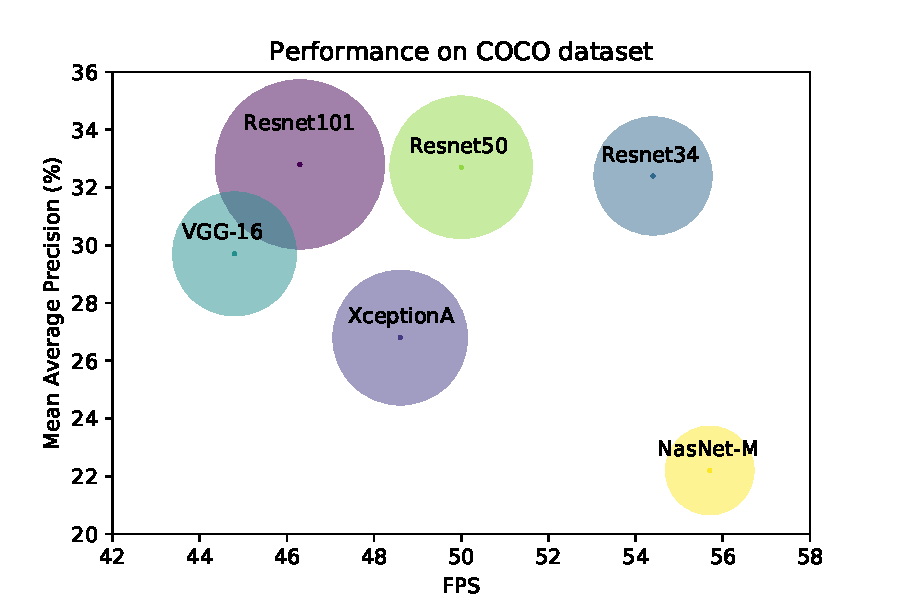
\includegraphics[width=0.975\textwidth]{img/fps_map_c}
    \caption[Performance of SSD with multiple base networks on COCO dataset]{Performance of SSD detector on multiple base networks. Circle radii demonstrate relative difference of network parameter counts. }
    \label{fig:cocoperf}
\end{figure}

\section{Training Data and Classes}
The principal difficulty in solving problems with neural networks is the lack of available data. Although some networks can be trained using reinforcement learning, object detection is one of those that requires supervision. However, the creation of a problem-specific dataset requires a lot of human resources. The other option is to use public datasets like the COCO dataset. 

The problem of such datasets is that if they include every required class, they also often include many classes that are not needed for a particular application. For surveillance, we are only interested in classes such as people and vehicles. 

We compared the performance and precision of SSD trained on full COCO dataset and a subset for surveillance. We expected significant performance improvement by lowering the number of detected classes. However, we were not sure how would this change impact precision. We hypothesized that by removing classes with similar features to the detected ones, there is a possibility of increasing the error by means of false detections.

\subsubsection{Surveillance Dataset Classes}
\begin{multicols}{2}
    \begin{itemize}
        \item person
        \item bicycle
        \item motorcycle
        \item car
        \item bus
        \item truck
        \item train
    \end{itemize}
\end{multicols}

\subsection{Precision Impact}
Before we get to the comparison of the training results, we will explain our hypothesis on an example. Consider that we want to detect people in a ZOO and we have access to the dataset with people and animals. Would it be better to train the network only to detect people or to detect both humans and animals, and then filter out the animals in post-processing? In the latter case, the network would ideally detect people as people, animals as animals, and everything else as a background. However, in the case where we train the network only to recognize people, how would such a network classify a monkey? Would similar features prevail and shift the classifier towards the person, or would negative examples of a monkey in dataset be strong enough for teaching the network that it is not a person? 

The problem we describe is, of course, part of a broader difficulty with non-exhaustive datasets. Our question is, therefore: If we have an available set of annotations for the classes we are not interested in, but that can be present in our input images and share similarities with detected classes, would it not be better to learn to detect those classes?

\subsubsection{Results}
\Cref{tab:ssdcocosurv} shows that in our case, it is possible to remove unnecessary classes from the dataset without impacting the performance. It is worth mentioning that we tried to precautiously counter-measure our hypothesis by creating the Surveillance dataset by only filtering the annotations and keeping all images of the original dataset.

We tested the approach on multiple architectures, and the results do not conclusively favor one dataset over the other. However, based on this experiment, we are not able to conclusively confirm or deny our hypothesis. Even if we wanted to make a conclusion for the COCO dataset using the provided training and validation data, the experiment is still dependant on the choice of classes.

\begin{table}
    \centering
    \begin{tabular}{c|c|c}
         & COCO & Surveillance  \\
         \hline
        ResNet34 & 47.3 & 47.3 \\
        ResNet50 & 46.6 & 48.7 \\
        ResNet101 & 47.2 & 45.7 \\
        XceptionA & 39.4 & 37.8 \\
        NASNet & 36.4 & 36.9 
    \end{tabular}
    \caption[SSD's precision comparison between COCO and Surveillance datasets]{Mean average precision of Surveillance classes. Comparing networks trained on all 80 classes of COCO dataset and Surveillance subset of COCO.}
    \label{tab:ssdcocosurv}
\end{table}

\subsection{Performance Impact}
We expected a proportional increase in performance with the elimination of unwanted classes. We saw in \cref{fig:VGGSSD} that the channel depth of the classification layers in SSD is dependent on the number of classes. Shallower classification layers are not only processed faster in the neural network but also produce less data that will result in faster post-processing, mainly, non-maximum suppression.

We illustrate the effect that the number of detected classes has on performance in \cref{fig:fpscls}. Although the relationship of frames per second and classes is hyperbolic, on the interval between 7 and 80 classes, we approximate the loss of 0.8fps with each additional class on ResNet50-SSD. Considering the dataset can contain tens or hundreds of classes, we showed that the filtering out the unwanted classes could produce significant performance benefit.

\begin{figure}
    \centering
    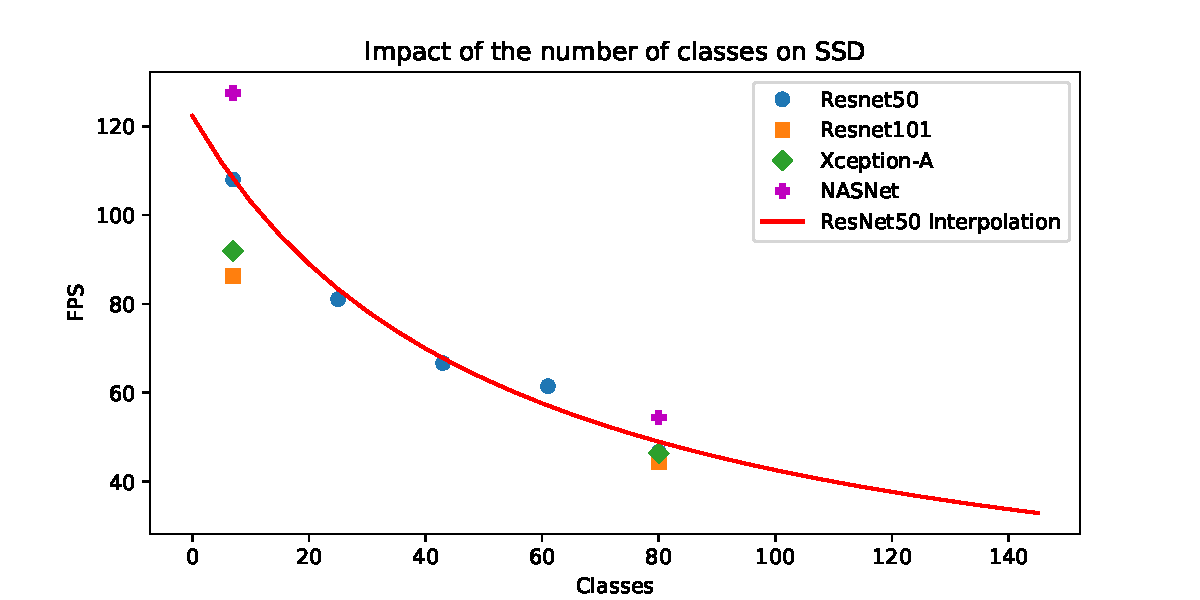
\includegraphics[width=\textwidth]{img/fps_cls}
    \caption[Impact of the number of classes on SSD performance]{Impact of the number of classes on SSD performance. Inference time values ($1/fps$) are linearly interpolated, the result is therefore hyperbolic approximation of frames per second.}
    \label{fig:fpscls}
\end{figure}


\section{Modifying Xception}
\label{sec:fixxception}
We managed to successfully re-implement SSD on other architectures and boost the speed of surveillance by removing unnecessary classes. We can confidently say that ResNet50-SSD with 48.7\% mAP and 108fps or ResNet34-SSD with 47.3\% mAP and 125fps outperform original SSD on VGG16 with 46.1\% mAP and 42fps. However, we believed that the underwhelming result of XceptionA-SSD could be used as a stepping stone and the results could be pushed further with modifications to the Xception architecture. 

We already mentioned the hypothesis that the major factor limiting the precision of XceptionA-SSD is the extraction of [37\x37] feature map after the second block of the network. To rectify this problem, we decided to make adjustments to the network, in such a way that we could extract [37\x37] feature map after \textit{block 7}, and keep the [19\x19] map after \textit{block 11} as previously dictated by network architecture. The reasoning behind choosing \textit{block 7} was that it is deep enough in the network and leaves four blocks between the feature map extractions. It is perhaps a bit arbitrary decision and blocks 6 or 8 would do just as well, or better.  In order to achieve the correct sizes of feature maps, we moved the max-pooling with stride 2 from \textit{block 3} to \textit{block 8}. This resulted in outputs of the \textit{block 2-7} to be the [37\x37] size and \textit{block 8} to output [19\x19] feature map. 

The proposed change to the pooling, and thus feature map sizes results in the increased complexity of the network as the [19\x19\x728] features now grew to the [37\x37\x728] size. To remedy this, we decreased the number of channels for concerned blocks to 256. We also decided to continue with trimming layers in the rest of the network. In the end, we got the [37\x37] map with 256 channels, [19\x19] map with 512 channels and [10\x10] map with 1024 channels. The architecture with highlighted changes is illustrated on \cref{fig:xceptionH_SSD}. 

Our modification not only helped to improve Xception-SSD to overcome VGG16, but we also outperformed ResNet50-SSD's 48.7\% mean average precision with 49.8 \% mAP. However, despite our best efforts to save computation, we managed to outperform XceptionA only slightly, by achieving 105fps. The relative performance of XceptionH based SSD to other SSDs using the Surveillance dataset can be seen on \cref{fig:surv_perf}.

\begin{figure}
    \centering
    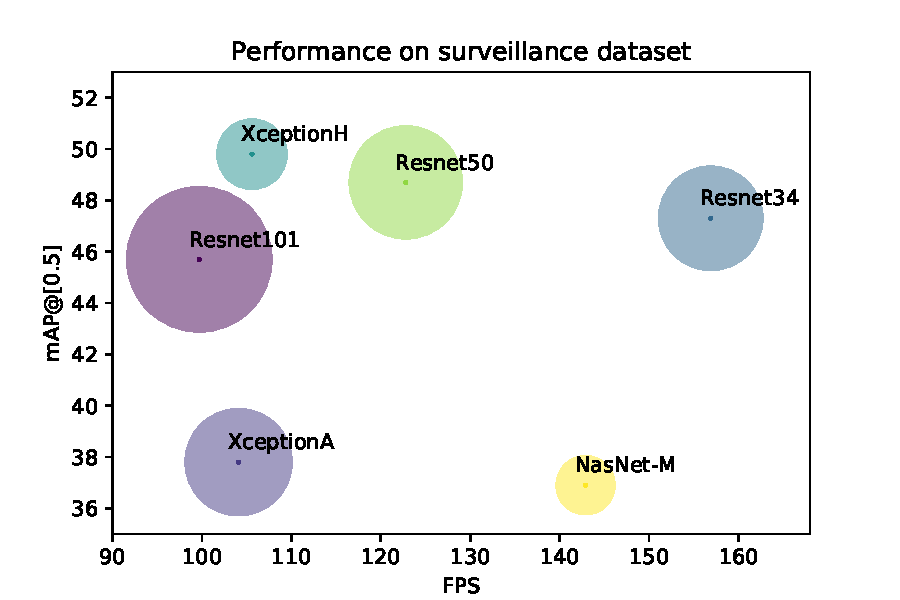
\includegraphics[width=\textwidth]{img/fps_map_s}
    \caption[Performance of SSD with multiple base networks on Surveillance dataset]{Performance of SSD detectors on multiple base networks on Surveillance dataset. Circle radii demonstrate relative difference of network parameter counts.} 
    \label{fig:surv_perf}
\end{figure}

\begin{figure}
    \centering
    \xceptionSSD
    \caption[XceptionH-SSD]%
    {XceptionH architecture (right) compared to XceptionA (left). Changes are highlighted with bold font. Connection to SSD's detection layers are indicated by the arrows on the sides, \textit{extra layers} are appended to the bottom of the network.  \textit{S} represents stride of the block, implemented using max-pooling. Blocks are also color-coded based on the feature map size. Extra, classification and localization layers are unchanged from \cref{fig:resnet_xception_SSD}. For details on \textit{Blocks} see \cref{fig:xception}.} 
    \label{fig:xceptionH_SSD}
\end{figure}


\section{SSDTC: SSD with Temporal Convolution}
\label{sec:ssdtc}
Since our main priority is video surveillance, we wanted to explore the options of video detection, exploiting the additional information a video can provide over still images. In \cref{sec:video_det} we have already examined two approaches of utilizing the continuity of video frames to achieve higher precisions. One approach used architecture similar to Faster R-CNN with use of temporal tubes-of-interest. The other one used convolutional LSTM cells to harness the temporal information inside a modified SSD. However, the major drawback of both approaches was their inference speed. 

Inspired by the two approaches, we decided to implement our version of video detector with temporal information. To this end, we chose to expand on the SSD. We already have an understanding of the model, and the one-stage detectors are currently the only relevant choice considering speed. We also wanted to avoid adding complex, time-consuming structures like LSTM cells used in TSSD. Instead, we decided to use three-dimensional convolutional layers (conv3d), to aggregate the information from multiple images. We named our approach \textit{Single Shot Detector with Temporal Convolution} (SSDTC).

Of course, we need to prove our concept by training it on some data and comparing it to unmodified SSD. Since we require a dataset with consecutive frames, we decided to start with the HollywoodHeads dataset. This set annotates heads in sections of movies. Considering that dataset has only one class and previous results of SSD testing suggests ResNet34-SSD would be more than sufficient for this task, we trained it as a baseline. Consequently, we also based SSDTC on ResNet34-SSD.

\subsubsection{Architecture}
In standard SSD, the detection is performed on a batch of independent images. We expect to perform detection on a single batch, or a chunk, of consecutive frames. 

We start by extracting the feature maps, as we would in SSD, independently on each frame with the same network (ResNet34 with \textit{extra layers}). Starting with the chunk \textit{n} = 16, we get 16 sets of feature maps. For the ease of explanation, consider only the first feature map of [38\x38\x c] size. Stacking those maps from the chunk, we get a temporal feature volume of [38\x38\x c\x n] size, where \textit{c} is the number of channels. 

At this point, we apply the temporal convolutional layers, realized using conv3d layers. We apply two conv3d layers on each feature volume, both followed by batch normalization and ReLU activation.  The first one, \textit{Conv3d. 1\x1\x3\x ch} operates only on temporal and channels dimensions.  The subsequent one works with all dimensions of feature volume, applying \textit{Conv3d. 3\x3\x3\x2*ch} layer. 

No padding is used in the temporal dimension of conv3d layers, therefore we only receive \textit{n-4} detections for \textit{n} input frames. This may seem inefficient because five frames are needed for detection on one frame, but the impact of this constant overhead can be minimized with bigger chunks. 

After the temporal layers, we can again view the created feature volume as an array of independent feature maps corespondent to frames and apply SSD's detection layers. 

In simple terms, we add temporal information from neighboring frames to each feature map, before executing the detection. This allows for reuse of most of the SSD's architecture and simple transition on other base networks. The illustration of SSDTC's architecture can be seen on \cref{fig:ssdtc}. To our best knowledge, this is a unique combination of SSD and three-dimensional convolution for object detection with temporal information.

\begin{figure}
    \centering
    \ssdtc
    \caption[Single Shot Detector with Temporal Convolution (SSDTC)]{SSDTC architecture on ResNet34 base. All temporal layers are followed by batch normalization and ReLU activation functions, no padding is used in temporal dimension.}
    \label{fig:ssdtc}
\end{figure}


\subsubsection{Results}
A previously mentioned, ResNet34-SSD was trained on the same dataset to serve as s baseline for comparison. This SSD achieved the precision of 81.16\% while performing at 156 frames per second. 

Our SSDTC architecture managed to reach the precision of 86.73\% with processing speed of 148 fps. However, considering that detection is not performed for every processed frame, the effective speed of the network is 111 frames per second with the chunk size of 16 frames. 
\todo{best on hheads?}
In \cref{fig:ssdssdtccomp}, we can see that SSDTC helped to remove many false detections and stabilized the detections.

\begin{figure}
    \centering
    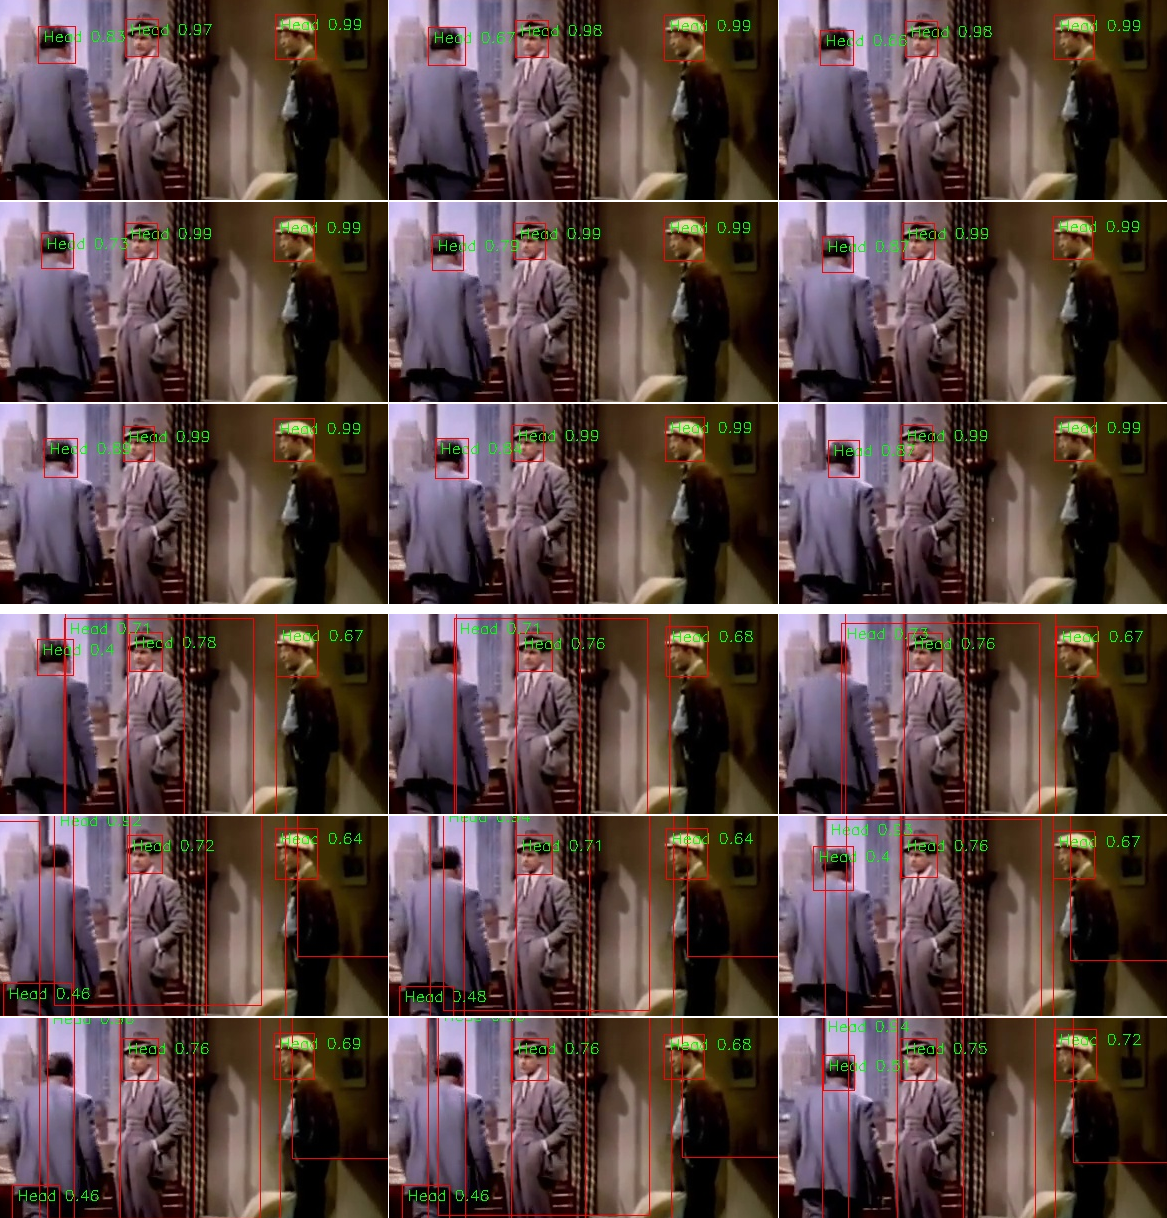
\includegraphics[width=\textwidth]{img/ssdt_ssdtc_comp}
    \caption[Comparison of detections by SSDTC and SSD]{Comparison of detections by SSDTC (top) and SSD (bottom). Performed on the sequence of nine frames, ordered from left to right, top to bottom. Frames were cropped after detection.}
    \label{fig:ssdssdtccomp}
\end{figure}